\phantomsection\section*{Введение}
\addcontentsline{toc}{section}{Введение}

В рамках педагогической практики были самостоятельно подготовлены и проведены два занятия по дисциплинам \enquote{мультимедиа-технологии} и \enquote{специальные главы математики}. Настоящий отчет включает в себя краткую характеристику самих занятий (план, цели и задачи, форма организации, список использованной литературы и т.д.), а также их результатов.

\begin{refsection}
\section{Занятие первое}

\subsection{Общая характеристика}

    \paragraph{Тема занятия.} \enquote{Методы анализа алгоритмов. Классы сложности $P$ и $NP$} по дисциплине \enquote{Мультимедиа-технологии}.

    \paragraph{Тип занятия.} Лекционное. Содержит материал о методах анализа алгоритмов на предмет корректности, эффективности, сложности, математических классах сложности и проблемах, связанных с ними ($P = NP$). Включает объяснение и изучение нового материала о классах сложности алгоритмов, методах их анализа, закрепление знаний об алгоритмах в целом, их возможных классификациях, а также контроль приобретаемых и имеющихся знаний.

    \paragraph{Цель занятия.} Организация познавательной деятельности студентов для усвоения ими новых теоретических знаний об алгоритмах, методах их анализа, математических классах сложности, совершенствования имеющихся базовых навыков анализа алгоритмов.

    \paragraph{Педагогические принципы.} Наглядности, научности, систематичности и последовательности, связи теории с практикой, сотрудничества, сознательности, активности и самодеятельности.

    \paragraph{Форма организации студентов.} Фронтальная.

    \paragraph{Средства обучения.} Компьютер с установленным программным обеспечением для просмотра презентаций, компьютерная презентация, проектор, экран.

\subsection{Задачи}

    \paragraph{Образовательные.} \begin{itemize}
        \item Закрепление базовых знаний об алгоритмах и задачах (понятие алгоритма, задачи, экземпляра задачи в различных формулировках).
        \item Закрепление знаний о простейших классификациях алгоритмов в рамках различных систем классификации.
        \item Закрепление знаний о базовых свойствах алгоритмов (дискретность, детерминированность, понятность и т.п.).
        \item Закрепление знаний о простейших методах анализа алгоритмической сложности.
        \item Ознакомление студентов с методами анализа алгоритмов на предмет их корректности. Краткая характеристика метода логических инвариантов, формальной верификации с помощью автоматизированных инструментов анализа на базе математической логики, других автоматических и полуавтоматических методов.
        \item Ознакомление студентов с понятиями машины Тьюринга и RAM-машины, их взаимосвязью и применением к анализу алгоритмической сложности.
        \item Объяснение студентам понятия математического класса сложности задачи. Знакомство с различными базовыми классами сложностями задач на конкретных примерах. Введение в проблематику \enquote{$P = NP$} с анализом данной математической проблемы и следствиями доказательства гипотезы $P = NP$.
        \item Формирование умений анализа задач на предмет определения класса сложности.
    \end{itemize}

    \paragraph{Воспитательные.} \begin{itemize}
        \item Воспитание коммуникативных навыков студентов посредством обсуждения поставленных преподавателем вопросов, общения с преподавателем.
        \item Мотивирование на дальнейшее развитие навыков формального анализа алгоритмов с использованием современных автоматизированных инструментов формальной верификации, анализ возникающих в рамках профессиональной деятельности задач с целью определения класса сложности задачи для выбора наиболее подходящего для ее решения алгоритма (класса алгоритмов), анализ самих алгоритмов на предмет их сложности с целью выбора наиболее подходящего по определенным критериям в конкретной ситуации.
        \item Побуждение к познавательной и научной деятельности.
    \end{itemize}

    \paragraph{Развивающие.} \begin{itemize}
        \item Развитие способности применять теоретические знания для практического анализа конкретных примеров.
        \item Развитие навыков работы и анализа получаемой посредством презентации информации.
        \item Развитие внимания через анализ студентами конкретных примеров с использованием изложенного материала.
    \end{itemize}

\subsection{Методы обучения}

    \paragraph{По источнику информации и восприятию.} \begin{itemize}
        \item Словесные (устное изложение теоретического материала, беседа и обсуждение вопросов).
        \item Наглядные (компьютерная презентация по теме лекции, в которой представлена графическая информация в виде схем, рисунков, формул, листингов алгоритмов, а также основные теоретические положения в кратком тезисном виде).
        \item Практические (анализ примеров из презентации совместно с преподавателем и самостоятельно).
    \end{itemize}

    \paragraph{По логике мышления.} \begin{itemize}
        \item Дедуктивные (анализ конкретных примеров задач и конкретных алгоритмов на основании изложенной общей теории сложности (математической и алгоритмической)).
        \item Индуктивные (теоретическое изложение следует от простых частных вопросов к общей связующей теории).
    \end{itemize}

    \paragraph{По степени самостоятельности и активности познавательной деятельности студентов.} \begin{itemize}
        \item Репродуктивные (систематизация имеющихся у студентов знаний об алгоритмах; краткая сводка нового материала перед началом работы над упражнениями).
        \item Проблемно-поисковые (студенты решают небольшие практические задачи по теме лекции, взаимодействуют с преподавателем).
        \item Исследовательские (студенты сравнивают различные задачи из разных классов сложности, анализируют последствия доказательства гипотезы $P = NP$ на базе имеющихся и полученных знаний).
    \end{itemize}

\subsection{Ход занятия}

\noindent\begin{longtable}{| p{.18\textwidth} | p{.41\textwidth} | p{.33\textwidth} |}\hline
    {\textbf{Этап занятия}} &
    {\textbf{Деятельность преподавателя}} &
    {\textbf{Деятельность студентов}} \\ \hline

    \multicolumn{3}{|c|}{Организационный момент} \\ \hline

    {} &
    {Представляется студентам. Формулирует тему лекции, ставит задачи, намеченные на предстоящее занятие} &
    {Знакомятся с преподавателем. Вспоминают пройденный материал, лежащий в основе занятия} \\ \hline

    \multicolumn{3}{|c|}{Объяснение нового материала} \\ \hline

    {Базовые сведения об алгоритмах} &
    {Вводит понятия алгоритма в различных трактовках, задачи и экземпляра задачи, объясняет основные свойства алгоритмов и их основные классификации, направления и цели анализа алгоритмов} &
    {Вспоминают известные сведения об алгоритмах и их классификациях, усваивают новые системные знания по данному вопросу} \\ \hline

    {Методы анализа корректности алгоритмов} &
    {В обзорном ключе объясняет возможные методы анализа корректности алгоритмов с упором на формальные методы анализа корректности (вручную и с использованием компьютерных систем). Предлагает студентам самостоятельно ознакомиться с некоторыми наиболее важными системами формальной верификации и статического анализа алгоритмов (с указанием источников информации). Проводит параллели между анализом алгоритмов (область математики и информатики) и анализом программного кода (область программирования, программной инженерии)} &
    {Заинтересовываются возможностью формальной верификации алгоритмов и статическим анализом программного кода автоматизированными программными средствами, теорией, лежащей в их основе. Задают вопросы о практическом применении указанных инструментов} \\ \hline

    {Понятие и методы анализа алгоритмической сложности} &
    {Раскрывает понятие алгоритмической (по времени, по памяти) сложности, связанные с этим понятия машины Тьюринга и RAM-машины, предположения, лежащие в основе анализа алгоритмической сложности, и способы анализа. Приводит простой пример расчета сложности для конкретного алгоритма (сортировки).} &
    {Вспоминают известные факты о сложности алгоритмов, необходимые математические сведения. Усваивают новый материал. Участвуют в разборе примера, задают вопросы о практической ценности анализа сложности алгоритмов} \\ \hline

    {Классы сложности} &
    {Вводит понятие класса сложности задачи, дает определения классам $P$, $NP$, $NPC$, $NPH$ в рамках единой взаимосвязанной системы, приводит примеры задач, попадающих в каждый из указанных классов с разбором причин} &
    {Усваивают новый материал о классах сложности, соотносят материал данного пункта с материалом предыдущего. Вместе с преподавателем разбирают конкретные примеры задач, пытаются определить их класс сложности} \\ \hline

    {Проблема \enquote{$P = NP$}} &
    {Ставит проблему доказательства гипотезы равенства классов $P$ и $NP$ и указывает на ее фундаментальную важность. Приводит возможные последствия (для математики, информатики, информационной безопасности и т.п.) доказательства этой гипотезы} &
    {Знакомятся с проблемой \enquote{$P = NP$}. Дополняют список возможных последствий равенства классов сложности $P$ и $NP$} \\ \hline

    \multicolumn{3}{|c|}{Контроль знаний} \\ \hline

    {Классы сложности} &
    {Предлагает студентам классифицировать набор задач, приведенный на слайдах презентации} &
    {Принимают совместное участие в решении поставленной задачи, участвуют в дискуссиях, обсуждают ошибки} \\ \hline
\end{longtable}

\subsection{Анализ занятия}

    Цели занятия были достигнуты~--- студентами были получены и усвоены необходимые знания по теме занятия. Поставленные дидактические задачи занятия были решены полностью.

    Выбранные методы, форма, средства обучения соответствуют типу и содержанию занятия. Наглядные, систематизированные и максимально сжатые материалы с большим количеством примеров улучшают восприятие сложного материала студентами. Фронтальная организация учащихся позволяет не только дать достаточно объемный материал в отведенное на занятие время, но и организовать взаимодействие с преподавателем в рамках совместного решения небольших задач по теме занятия. Это позволяет, с одной стороны, осуществить контроль получаемых знаний, оценить степень вовлеченности студентов в тему занятия, дать возможность студентам проявить себя, с дугой стороны, не отвести излишне много времени на самостоятельное решение задач и последующую (совместную) проверку решений.

    В ходе занятия студенты выглядели серьезными, заинтересованными излагаемым материалом. Они внимательно слушали преподавателя, принимали участие в дискуссиях, отвечали на вопросы преподавателя и задавали свои. Студенты выражали желание более глубоко ознакомиться с отдельными вопросами занятия, возможностью применения излагаемого материала в учебной и профессиональной деятельности.

    Отведенное на занятие время и сложность некоторых вопросов занятия послужили ограничивающим фактором для более полного и глубокого раскрытия материала. Это не повлияло на его системность и общность, а также на наличие большого количества практических примеров и упражнений для студентов. Некоторые вопросы занятия были вынужденно сделаны сугубо обзорными, однако студентам был предоставлен прокомментированный список рекомендованной литературы для более глубокого ознакомления с теорией и практикой по этим вопросам.

\nocite{*}\printbibliography[heading=lessonbib, keyword={lesson1}]

\end{refsection}

\begin{refsection}
\section{Занятие второе}

\subsection{Общая характеристика}

    \paragraph{Тема занятия.} \enquote{Обратные задачи: условия корректности, обратные задачи матфизики, экстремальные задачи для выпуклого функционала} по дисциплине \enquote{Специальные главы математики}.

    \paragraph{Тип занятия.} Лекционное. Включает систематизацию и закрепление знаний об обратных задачах в целом, условиях их корректности, объяснение и изучение нового материала о выпуклых функционалах, функциях и множествах, классификацию обратных задач математической физики и теории систем, обзор некоторых обратных задач математической физики.

    \paragraph{Цель занятия.} Организация познавательной деятельности студентов для усвоения ими новых теоретических знаний об обратных задачах, выпуклых функционалах, множествах, функциях.

    \paragraph{Педагогические принципы.} Наглядности, научности, систематичности и последовательности, сознательности.

    \paragraph{Форма организации студентов.} Фронтальная.

    \paragraph{Средства обучения.} Компьютер с установленным программным обеспечением для просмотра презентаций, компьютерная презентация, проектор, экран.

\subsection{Задачи}

    \paragraph{Образовательные.} \begin{itemize}
        \item Закрепление базовых знаний об обратных задачах (понятие обратной задачи, корректность задачи, условия корректности задачи).
        \item Ознакомление студентов с понятиями выпуклого множества, функции, функционала, оптимизацией выпуклых функций, функционалов, операторами проекций на выпуклые множества как инструментом итерационного решения задачи с ограничениями.
        \item Объяснение студентам классификации обратных задач с точки зрения теории систем.
        \item Ознакомление студентов с некоторыми обратными задачами математической физики (на примере одномерного уравнения теплопроводности).
        \item Формирование умений анализа задач на предмет корректности согласно условиям корректности.
    \end{itemize}

    \paragraph{Воспитательные.} \begin{itemize}
        \item Мотивирование на дальнейшее развитие навыков решения обратных задач с ограничениями с помощью аппарата выпуклых множеств и функционалов там, где это применимо.
        \item Побуждение к познавательной и научной деятельности.
    \end{itemize}

    \paragraph{Развивающие.} \begin{itemize}
        \item Развитие навыков работы и анализа получаемой посредством презентации информации.
        \item Развитие внимания через анализ студентами конкретных примеров (обратных задач) с использованием изложенного материала (классификации обратных задач, условий корректности).
    \end{itemize}

\subsection{Методы обучения}

    \paragraph{По источнику информации и восприятию.} \begin{itemize}
        \item Словесные (устное изложение теоретического материала).
        \item Наглядные (компьютерная презентация по теме лекции, в которой представлена графическая информация в виде схем, рисунков, формул, а также основные теоретические положения в кратком тезисном виде).
        \item Практические (анализ примеров из презентации совместно с преподавателем).
    \end{itemize}

    \paragraph{По логике мышления.} \begin{itemize}
        \item Дедуктивные (анализ конкретных примеров (обратных задач) на основании изложенной общей теории (классификации, условий корректности)).
    \end{itemize}

    \paragraph{По степени самостоятельности и активности познавательной деятельности студентов.} \begin{itemize}
        \item Репродуктивные (систематизация имеющихся у студентов знаний об обратных задачах, условиях их корректности).
        \item Проблемно-поисковые (студенты решают небольшие практические задачи по теме лекции, взаимодействуют с преподавателем).
    \end{itemize}

\subsection{Ход занятия}

\noindent\begin{longtable}{| p{.18\textwidth} | p{.41\textwidth} | p{.33\textwidth} |}\hline
    {\textbf{Этап занятия}} &
    {\textbf{Деятельность преподавателя}} &
    {\textbf{Деятельность студентов}} \\ \hline

    \multicolumn{3}{|c|}{Организационный момент} \\ \hline

    {} &
    {Представляется студентам. Формулирует тему лекции, ставит задачи, намеченные на предстоящее занятие} &
    {Знакомятся с преподавателем. Вспоминают пройденный материал, лежащий в основе занятия} \\ \hline

    \multicolumn{3}{|c|}{Объяснение нового материала} \\ \hline

    {Выпуклые функции, функционалы, множества, операторы проекции на выпуклые множества} &
    {Вводит понятия выпуклой функции, функционала, множества. Приводит определение задачи условной оптимизации для функции (функционала) в общем и для выпуклой функции (функционала) в частности. Формулирует понятие оператора проекции на выпуклые множества, сужающего оператора, его фиксированной точки как (итерационного) решения задачи с ограничениями} &
    {Вспоминают известные сведения о задачах оптимизации. Усваивают новый материал о выпуклых функциях, операторах проекции на выпуклые множества. Задают вопросы о практической применимости излагаемых методов, способах определения выпуклости функции (множества). Заинтересовываются возможностью упрощения анализа задачи оптимизации применением к ней аппарата выпуклых функций и множеств} \\ \hline

    {Обратные задачи в теории систем и математической физике} &
    {Объясняет классификацию обратных задач с точки зрения теории систем. Приводит примеры обратных задач теории систем и математической физики. Разбирает конкретные примеры со студентами} &
    {Усваивают классификацию обратных задач теории систем и математической физики, участвуют в обсуждении примеров} \\ \hline

    {Корректность обратных задач} &
    {Вводит понятие корректной задачи, условия корректности задачи, приводит связь некорректных и обратных задач, примеры задач, не удовлетворяющих тем или иным критериям корректности} &
    {Вспоминают известные сведения о некорректных и обратных задачах, участвуют в обсуждении примеров некорректных задач} \\ \hline
\end{longtable}

\subsection{Анализ занятия}

    \begin{figure}[h]
        \centering
        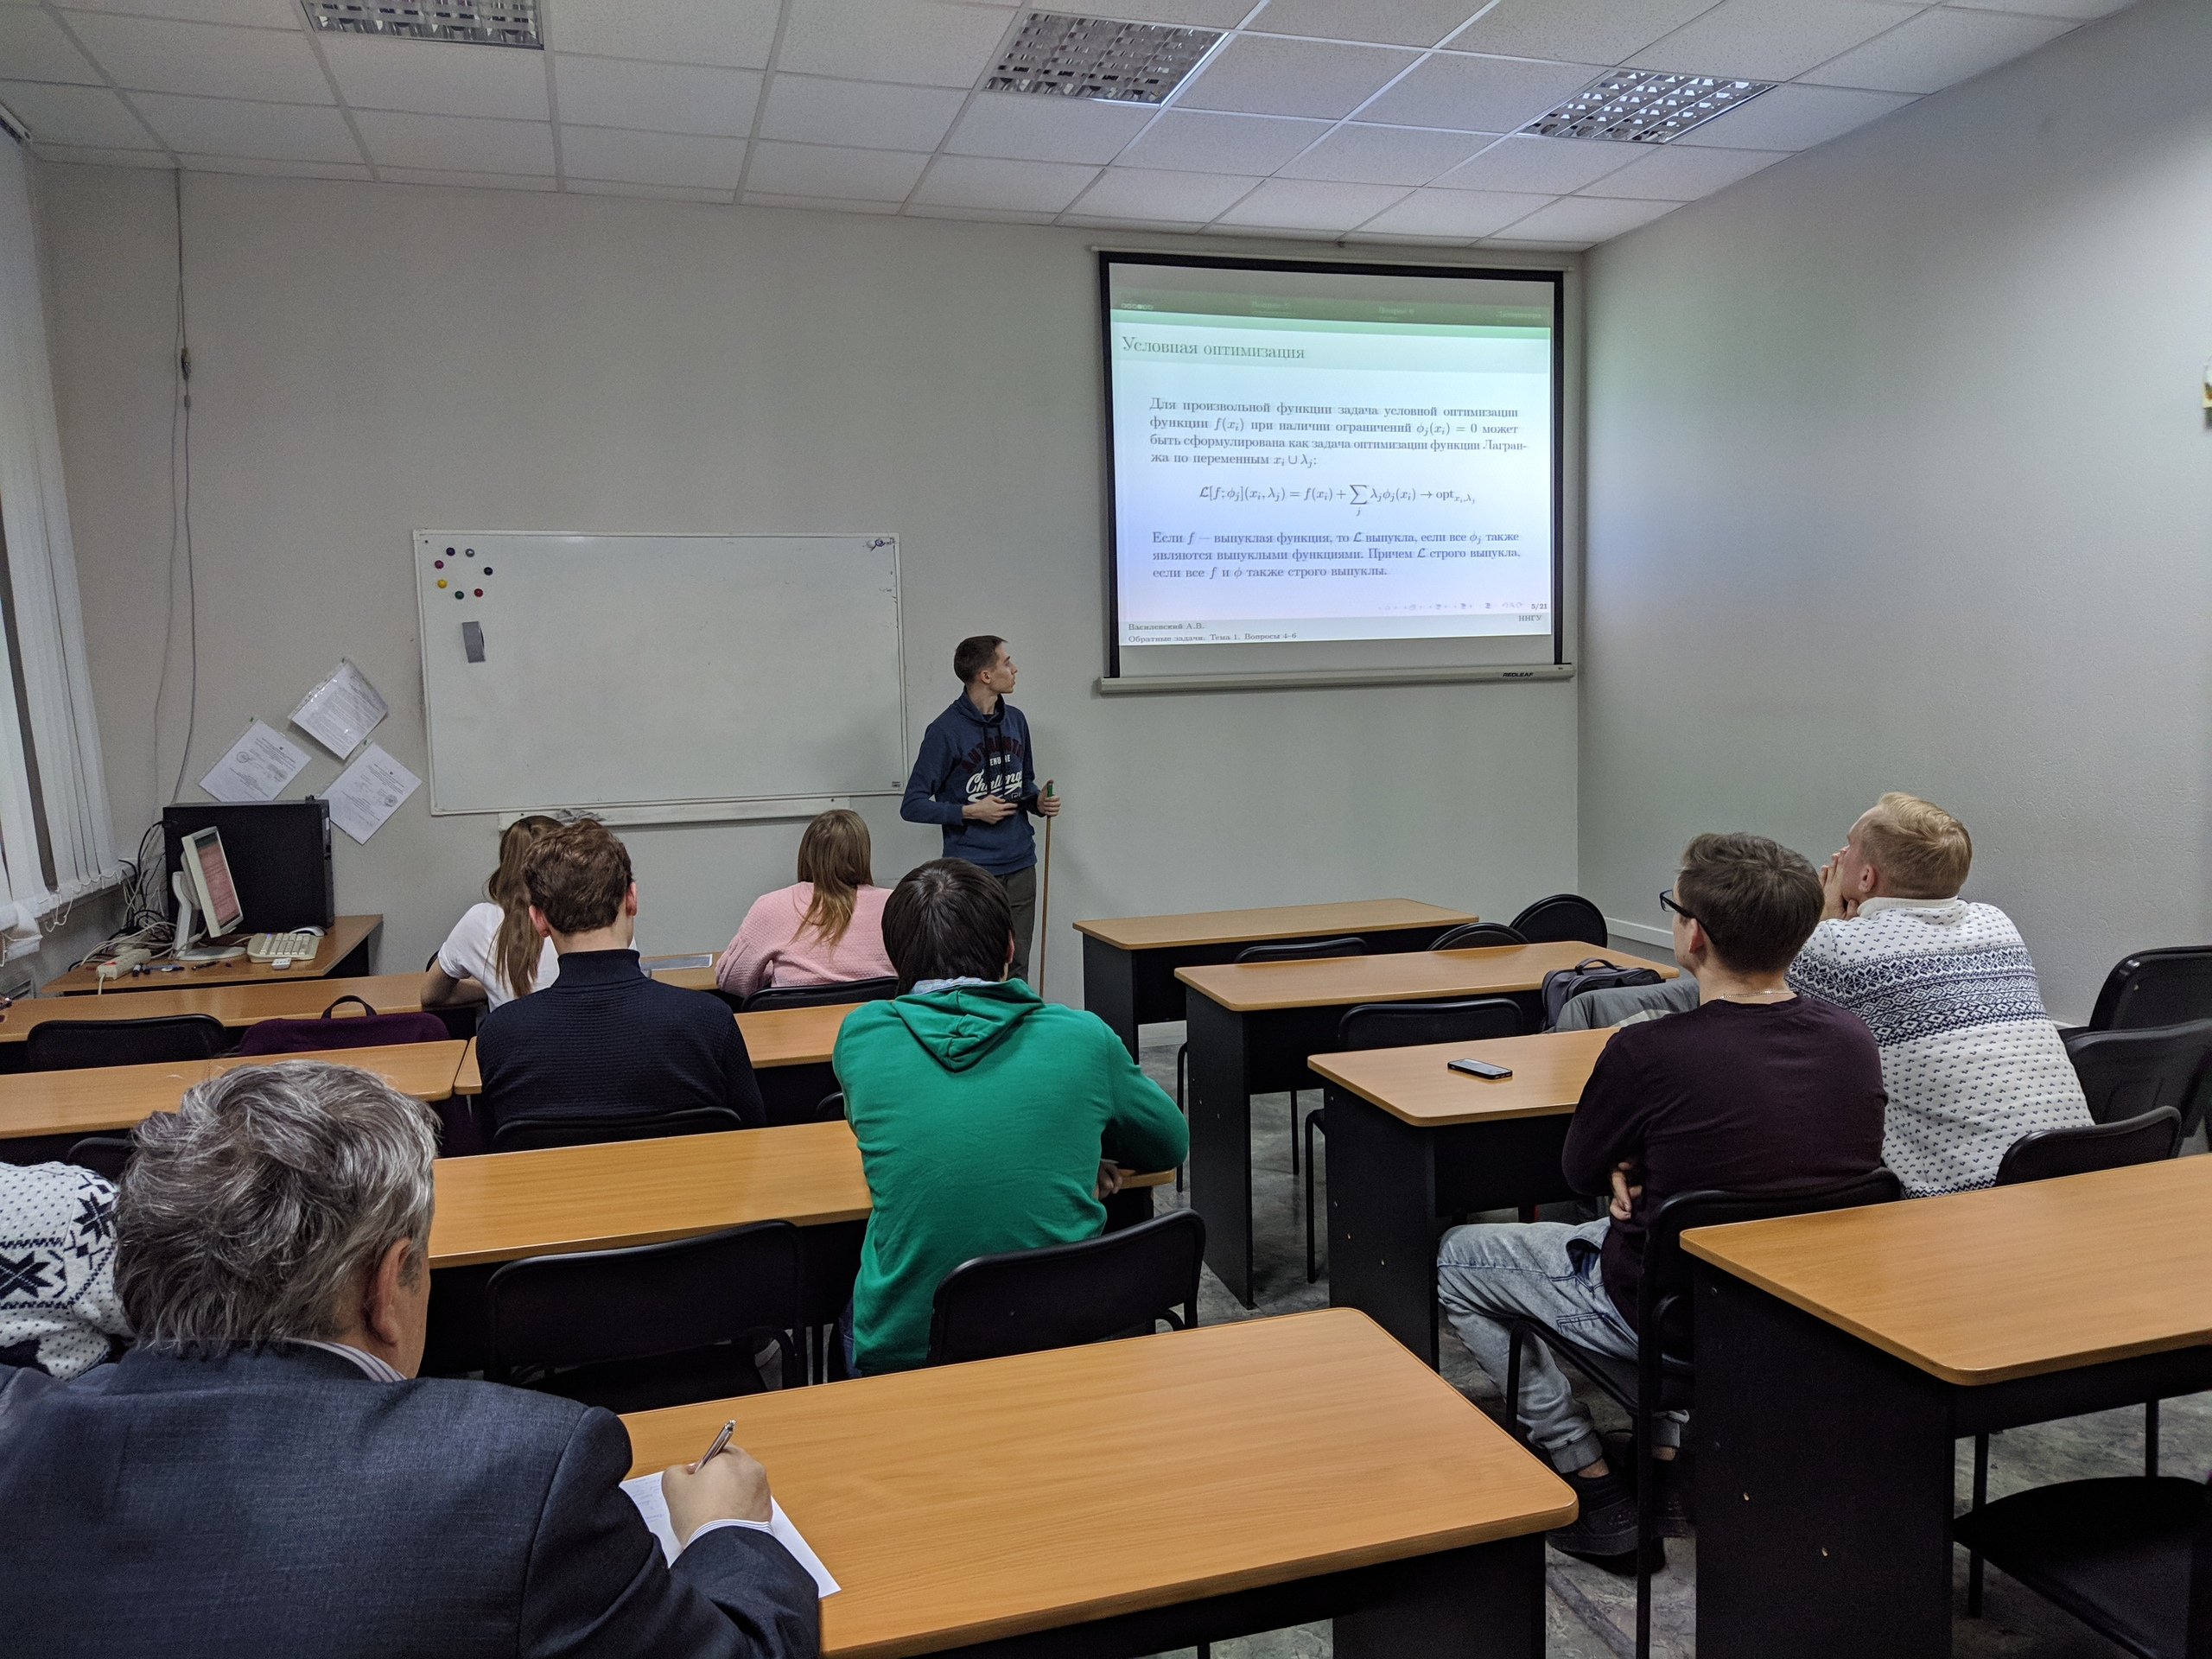
\includegraphics[width=\textwidth]{witness.jpg}
        \caption{Преподаватель объясняет студентам один из вопросов занятия}
    \end{figure}

    Цели занятия были достигнуты~--- студенты получили и усвоили новые знания по теме занятия. Поставленные дидактические задачи были решены.

    Выбранные методы, форма, средства обучения соответствуют типу и содержанию занятия. Наглядные материалы улучшают восприятие материала студентами, способствуют лучшему запоминанию и усвоению информации. Фронтальная организация учащихся позволяет максимально раскрыть тему занятия и дать наиболее полную и общую информацию по теме за отведенное на занятие время.

    В ходе занятия студенты выглядели серьезными, интересующимися темой занятия и мотивированными на дальнейшее и более полное изучение и практическое применение полученных базовых знаний. Они внимательно слушали преподавателя, участвовали в обсуждении приводимых примеров, по окончании занятия задавали вопросы и беседовали с преподавателем по теме занятия.

    При подготовке занятия преподаватель столкнулся с рядом трудностей, обусловленных, в основном, необходимостью уложить достаточно объемный и многогранный материал в отведенное на занятие время. В процессе составления плана занятия приходилось ограничивать количество менее существенной информации, не жертвуя при этом полнотой и понятностью изложения и дополняя сугубо теоретический материал его возможными практическими применениями к знакомым студентам задачам (обработка сигналов, восстановление изображений, задачи оптимизации и оптимального управления и т.д.).

\nocite{*}\printbibliography[heading=lessonbib, keyword={lesson2}]

\end{refsection}

\phantomsection\section*{Выводы}
\addcontentsline{toc}{section}{Выводы}

Оба проведенных занятия соответствуют целям занятия, все из которых были достигнуты в процессе проведения занятий. В ходе занятий студенты проявляли активность, заинтересованность, выказывали понимание излагаемого материала. При подготовке занятий преподаватель не столкнулся с какими-либо серьезными сложностями, за исключением необходимости дать студентам сложный и объемный материал в отведенное на занятие время, сделать его доступным студентам.
